\documentclass{standalone}
\usepackage{fontspec}
\setsansfont{Arial}
\usepackage{tikz}
\usetikzlibrary{arrows.meta,positioning}
\tikzset{every picture/.append style={font=\sffamily\footnotesize}}
\begin{document}
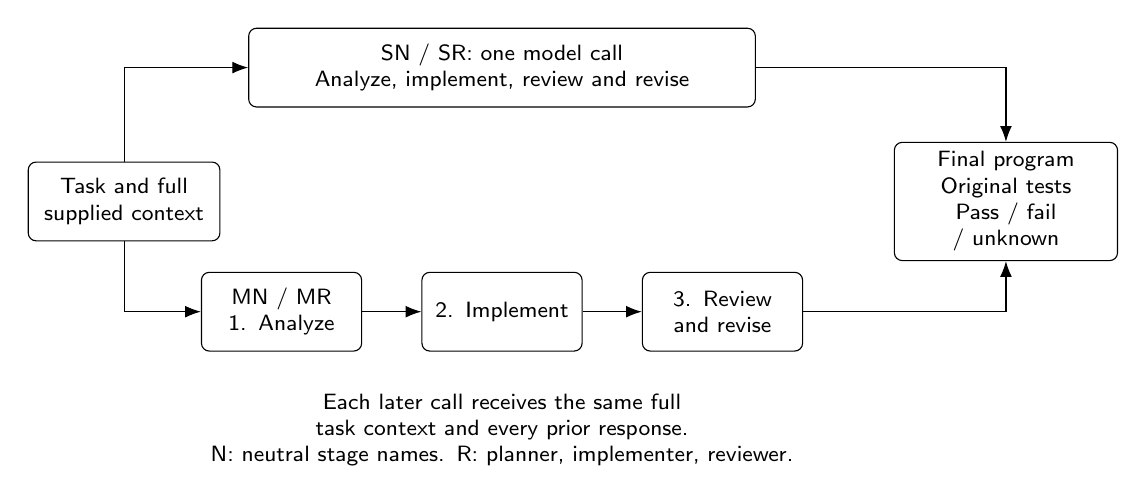
\begin{tikzpicture}[x=1mm,y=1mm,
box/.style={draw,rounded corners=1mm,align=center,text width=28mm,minimum height=10mm},
flow/.style={-{Latex[length=2mm]}}]
\node[box,text width=22mm] (input) at (0,0) {Task and full\\supplied context};
\node[box,text width=62mm] (single) at (48,17) {SN / SR: one model call\\Analyze, implement, review and revise};
\node[box,text width=18mm] (plan) at (20,-14) {MN / MR\\1. Analyze};
\node[box,text width=18mm] (code) at (48,-14) {2. Implement};
\node[box,text width=18mm] (review) at (76,-14) {3. Review\\and revise};
\node[box,text width=26mm] (test) at (112,0) {Final program\\Original tests\\Pass / fail / unknown};
\draw[flow] (input.north) |- (single.west);
\draw[flow] (input.south) |- (plan.west);
\draw[flow] (plan) -- (code); \draw[flow] (code) -- (review);
\draw[flow] (single.east) -| (test.north);
\draw[flow] (review.east) -| (test.south);
\node[align=center,text width=92mm] at (48,-29) {Each later call receives the same full task context and every prior response.\\N: neutral stage names. R: planner, implementer, reviewer.};
\end{tikzpicture}
\end{document}
